\documentclass[]{beamer}
\mode<presentation> {
	
	% The Beamer class comes with a number of default slide themes
	% which change the colors and layouts of slides. Below this is a list
	% of all the themes, uncomment each in turn to see what they look like.
	
	%\usetheme{default}
	%\usetheme{AnnArbor}
	%\usetheme{Antibes}
	%\usetheme{Bergen}
	\usetheme{Berkeley}
	%\usetheme{Berlin}
	%\usetheme{Boadilla}
	%\usetheme{CambridgeUS}
	%\usetheme{Copenhagen}
	%\usetheme{Darmstadt}
	%\usetheme{Dresden}
	%\usetheme{Frankfurt}
	%\usetheme{Goettingen}
	%\usetheme{Hannover}
	%\usetheme{Ilmenau}
	%\usetheme{JuanLesPins}
	%\usetheme{Luebeck}
	%\usetheme{Madrid}
	%\usetheme{Malmoe}
	%\usetheme{Marburg}
	%\usetheme{Montpellier}
	%\usetheme{PaloAlto}
	%\usetheme{Pittsburgh}
	%\usetheme{Rochester}
	%\usetheme{Singapore}
	%\usetheme{Szeged}
	%\usetheme{Warsaw}
	
	% As well as themes, the Beamer class has a number of color themes
	% for any slide theme. Uncomment each of these in turn to see how it
	% changes the colors of your current slide theme.
	
	%\usecolortheme{albatross}
	%\usecolortheme{beaver}
	%\usecolortheme{beetle}
	%\usecolortheme{crane}
	%\usecolortheme{dolphin}
	%\usecolortheme{dove}
	%\usecolortheme{fly}
	%\usecolortheme{lily}
	%\usecolortheme{orchid}
	%\usecolortheme{rose}
	%\usecolortheme{seagull}
	%\usecolortheme{seahorse}
	%\usecolortheme{whale}
	%\usecolortheme{wolverine}
	
	%\setbeamertemplate{footline} % To remove the footer line in all slides uncomment this line
	%\setbeamertemplate{footline}[page number] % To replace the footer line in all slides with a simple slide count uncomment this line
	
	%\setbeamertemplate{navigation symbols}{} % To remove the navigation symbols from the bottom of all slides uncomment this line
}

\usepackage[utf8]{inputenc} % codificacao de caracteres
\usepackage[T1]{fontenc}    % codificacao de fontes
\usepackage[brazil]{babel}  % idioma
\usepackage{listings}
\usepackage{color}
\usefonttheme[onlymath]{serif} % fonte modo matematic
\usepackage{adjustbox}
\usepackage{ragged2e}
\definecolor{gray}{rgb}{0.4,0.4,0.4}
\definecolor{darkblue}{rgb}{0.0,0.0,0.6}
\definecolor{cyan}{rgb}{0.0,0.6,0.6}

\lstset{
	basicstyle=\ttfamily,
	columns=fullflexible,
	showstringspaces=false,
	commentstyle=\color{gray}\upshape
}

\lstdefinelanguage{XML}
{
	morestring=[b]",
	morestring=[s]{>}{<},
	morecomment=[s]{<?}{?>},
	stringstyle=\color{black},
	identifierstyle=\color{darkblue},
	keywordstyle=\color{cyan},
	morekeywords={xmlns,version,type}% list your attributes here
}


%Titulo
\title[\sc{Static Analisys}]{\textbf{Análise estática para detectar a evoulução da
linguagem java em projetos open source}}
\author[Thiago Cavalcanti - Vinícius Correa]{Thiago Gomes Cavalcanti \\ Vinícius Correa de Almeida}

\institute{
	\includegraphics[scale=0.6]{as_comp_cor.eps}\\
	\textbf{Orientador: Prof. Dr. Rodrigo Bonifácio de Almeida}
}
\date[04/03/2016]{04 de março de 2016}

\begin{document}
	\begin{frame}
		\titlepage
	\end{frame}
	
	\begin{frame}
		\frametitle{Roteiro}
		\tableofcontents
	\end{frame}

	
%%%%%%%%%%%%%%%%%%%%%%%%%%% CENÁRIO %%%%%%%%%%%%%%%%%%%%%%%%%%%
	\section{Cenário}
	\begin{frame}[label=problems]
		\frametitle{O Software}
		\begin{itemize}
			\item Software atual com construções ultrapassadas.
			\item Código de baixa qualidade e difícil entendimento.
			\item Dificuldade em efetuar refactoring e testes.
			\item Desenvolvedores não conhecem de novas features da linguagem.
			\item A release não é importante no desenvolvimento.
			\item Time que está ganhando não se mexe!!!
		\end{itemize}
	\end{frame}
%%%%%%%%%%%%%%%%%%%%%%%%%%% CENÁRIO %%%%%%%%%%%%%%%%%%%%%%%%%%%



%%%%%%%%%%%%%%%%%%%%%%%%%%% MOTIVAÇÃO %%%%%%%%%%%%%%%%%%%%%%%%%%%
	\section{Motivação}
	
	\begin{frame}[label=Motivação]
		\frametitle{Motivação}
		\begin{block}{Fortran}
			\begin{itemize}
				\item Artigo Regrowing a Language de Jeffrey L. Overbey e Ralph E. Johnson.
				
				\item Remoção do ultrapassado estilo \textit{do loop} caso este terminasse com \textit{continue}, era substituído por construção equivalente \textit{end do}.
				
				\item Remoção do \textit{goto} por uma construção \textit{case} equivalente.
				
				\item Uso de palavras reservadas \textit{if, while, ...}, como variáveis.
				
				\item Introdução de OO em Fortran 2003.
			\end{itemize}
		\end{block}
	\end{frame}
	
		
	\begin{frame}[label=AspectosAnalisados]
		\frametitle{Aspectos analisados}
		\begin{block}{Aspectos Analisados}
			\begin{itemize}
				\item Investigação empíraca da adoção de features Java.
				
				\item Replicação de um estudo existente de Parnin et al.
				
				\item Investigou-se as características:
					\begin{itemize}
						\item \texttt{Generics}.
						\item \texttt{Lambda Expression}.
						\item \texttt{Multi-catch}.
						\item \texttt{Try-Resource}.
						\item \texttt{Switch-Stgring}.
					\end{itemize}

				\item Oportunidade de evolução em:
					\begin{itemize}
						\item \texttt{Lambda Expression}, \texttt{foreach, exists}.
						\item \texttt{Multi-catch}, \texttt{catch(E1 | E2 | ...)}.
					%	\item \texttt{Try-Resource}, \texttt{java.lang.AutoCloseable} ou \texttt{java.io.Closeable}.
						\item \texttt{Switch-String}, \textit{if(string.equals(""))}.
					\end{itemize}

			\end{itemize}
		\end{block}
	\end{frame}
	

	

	
%	\begin{frame}[label=DimensaoTrabalhos]
%		\frametitle{Dimensões Alcancáveis}
%		\begin{itemize}
%			\item Falar da pretenção do analisador estático reduzir custo no desenvolvimento.
%			\item E de como pode ajudar a ORACLE a tornar mais limpa as releases.
%			
%		\end{itemize}
%	\end{frame}
%%%%%%%%%%%%%%%%%%%%%%%%%%% MOTIVAÇÃO %%%%%%%%%%%%%%%%%%%%%%%%%%%	



%%%%%%%%%%%%%%%%%%%%%%%% Revisão teórica %%%%%%%%%%%%%%%%%%%%%%%%
	\section{Revisão Teórica}
	\frametitle{Referências}
	\begin{frame}[label=referencias]
		\begin{block}{Referências}
			\begin{itemize}
				\item Chris Parnin, Christian Bird, and Emerson Murphy-Hill 2011. \textbf{Java generics adoption: How new features are introduced, championed, or ignored}.
				
				\item Jefrey L. Overbey and Ralph E. Johnson. \textbf{Regrowing a language: refactoring tools
				allow programming languages to evolve}.
				
				\item Dyer, Robert and Rajan, Hridesh and Nguyen, Hoan Anh and Nguyen, Tien N. \textbf{Mining billions of AST nodes to study actual and potential usage of Java language features}.
			\end{itemize}
			
		\end{block}
	\end{frame}
	
%%%%%%%%%%%%%%%%%%%%%%%% Revisão teórica %%%%%%%%%%%%%%%%%%%%%%%%




%%%%%%%%%%%%%%%%%%%%% Diretrizes da pesquisa %%%%%%%%%%%%%%%%%%%%
	\section{Diretrizes da pesquisa}

	\begin{frame}[fragile]\frametitle{Problema}
		\begin{block}{Problema}
			\begin{itemize}
				\item Desenvolver um analisador estático de código Java.
			
				\item Pesquisar características ultrapassadas em projetos atuais.
			
				\item Refazer estudo de \texttt{Generis}.
			\end{itemize}
		\end{block}
	\end{frame}	
	
	
	\begin{frame}[fragile]\frametitle{Hipóteses}
		
	%	\begin{description}\item[\textbf{Hipótese 1}]\end{description}
		\begin{block}{Hipótese 1}
			\begin{itemize}
				\item Novas características são pouco utilizadas ou ignoradas no desenvolvimento do software.
			\end{itemize}
		
		\end{block}
		
		%\begin{description}\item[\textbf{Hipótese 2}]\end{description}
		\begin{block}{Hipótese 2}
			\begin{itemize}
				\item Código obsoleto é mantido em releases atuais.
			\end{itemize}
		\end{block}
		
	%	\begin{description}	\item[\textbf{Hipótese 3}]\end{description}
%		\begin{block}{Hipótese 3}
%			\begin{itemize}
%				\item Versões mais recentes do software não possem as últimas características adotadas na linguagem.
%			\end{itemize}
%		\end{block}
		
	\end{frame}
	
	
	\begin{frame}[fragile]\frametitle{Objetivos}
		%\begin{description}	\item[\textbf{Objetivo Geral}]\end{description}
		\begin{block}{Geral}
			\begin{itemize}
				\item Identificar de forma eficiente construções na linguagem Java.
			\end{itemize}
		\end{block}
			
		%\begin{description}	\item[\textbf{Objetivo Geral}]\end{description}
			\begin{block}{Específicos}
				\begin{itemize}
					\item Elaborar um analisador estático flexível.
				\end{itemize}
			\end{block}
	\end{frame}
%%%%%%%%%%%%%%%%%%%%% Diretrizes da pesquisa %%%%%%%%%%%%%%%%%%%%%
	
%%%%%%%%%%%%%%%%%%%%%%%%%%%% Metodologia %%%%%%%%%%%%%%%%%%%%%%%%%%%%%%%%%%%%%%%
	\section{Metodologia}
	\begin{frame}[label=metodologia, fragile]
		\frametitle{Procedimentos}
		\begin{block}{Ordem das tarefas}
			\begin{itemize}
				\item Revisão Bibliográfica
					\begin{itemize}
						\item Seleção do projetos.
						\item Escolha de projetos opensource.
					\end{itemize}
				\item Implementação do analisador estático.
					\begin{itemize}
						\item Definir arquitetura.
						\item Implementação.
						\item Coleta de dados.
					\end{itemize}
					
				\item Refazer os passos do artigo de Generics(escrever artigo).
			
				\item Contribuições adicionais.
			\end{itemize}
		\end{block}
	\end{frame}
	
		
%%%%%%%%%%%%%%%%%%%%%%%%%%%% Metodologia %%%%%%%%%%%%%%%%%%%%%%%%%%%%%%%%%%%%%%%
	

%%%%%%%%%%%%%%%%%%%%%%%%%%%%% ANALISADOR ESTÁTICO %%%%%%%%%%%%%%%%%%%%%%%%%%%%%%
\section{Arquitetura e Funcionamento Analisador Estático}


\begin{frame}[label=metodologia, fragile]
	\frametitle{Analisador Estático}
	\begin{block}{Classes Utilitárias}
			\begin{figure}[h]
				\center
				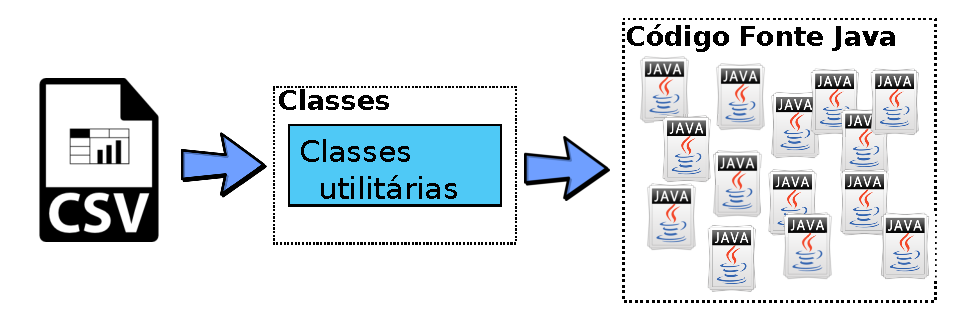
\includegraphics[scale=0.50]{../TCC/Imagens/InputArquitetura}
				\label{fig:oportunidadesSwitchString}
				\caption{Classes Utilitárias.}
			\end{figure}
	\end{block}
\end{frame}


\begin{frame}[label=metodologia, fragile]
	\frametitle{Analisador Estático}
	\begin{block}{Arquitetura}
			\begin{figure}[h]
				\center
				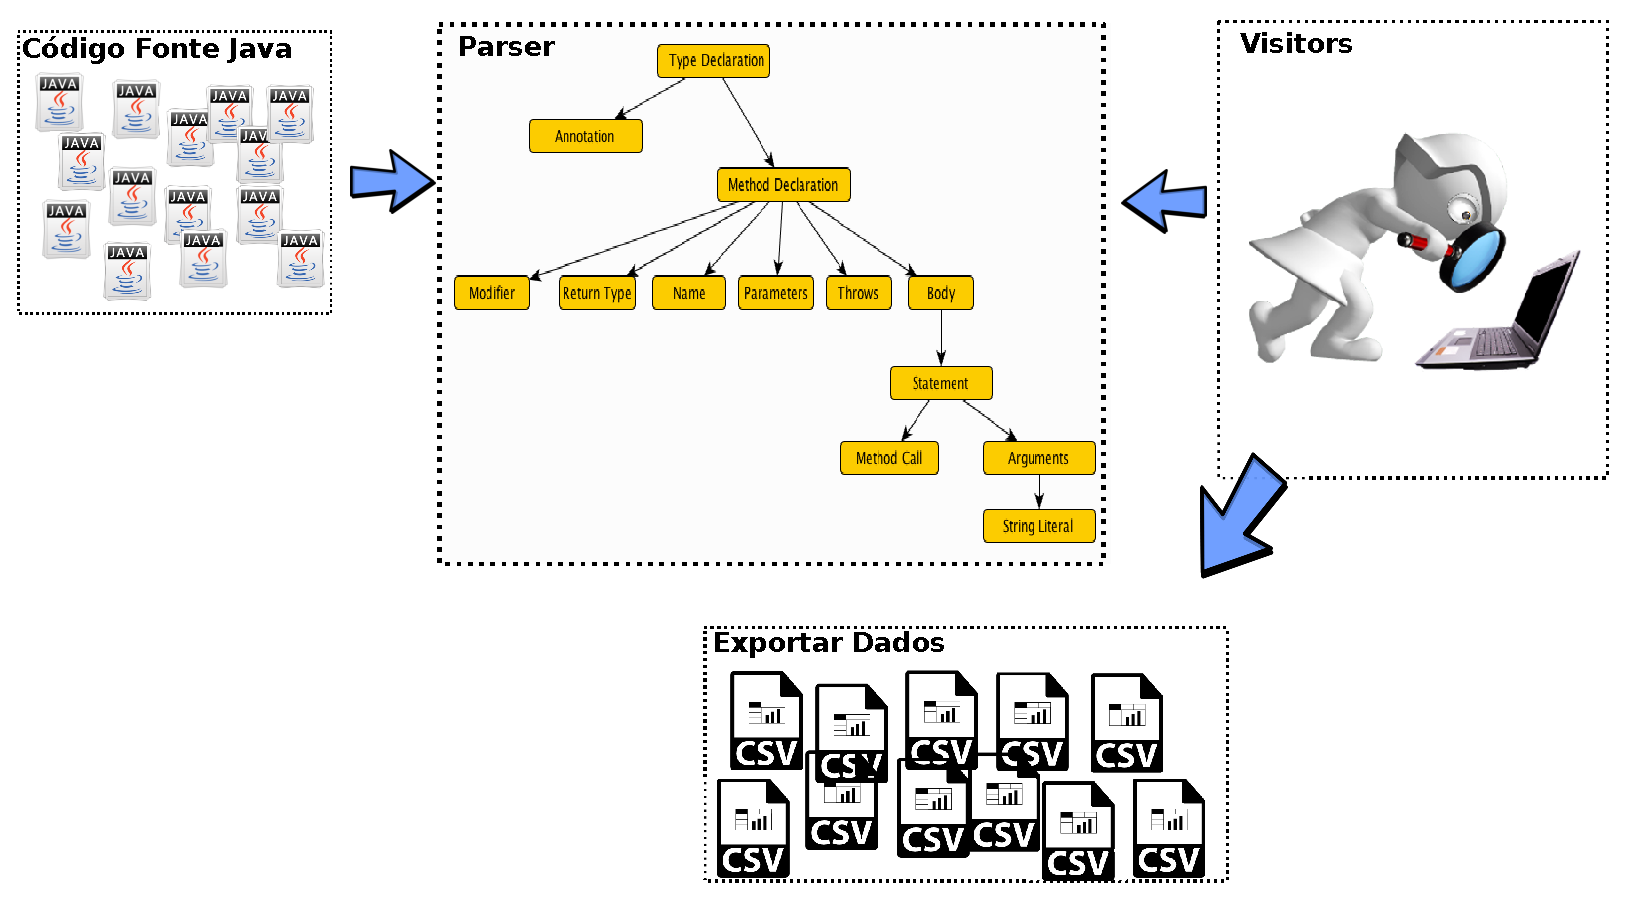
\includegraphics[scale=0.30]{../TCC/Imagens/FuncionamentoVisitor}
				\label{fig:oportunidadesSwitchString}
				\caption{Funcionamento Analisador Estático.}
			\end{figure}
	\end{block}
\end{frame}

	
	

%%%%%%%%%%%%%%%%%%%%% Resultados %%%%%%%%%%%%%%%%%%%%%
	\section{Resultados}
	
	\begin{frame}[fragile, label=re]\frametitle{Resultados}
		\begin{block}{Generics}
			\begin{itemize}
				\item 16\% dos projetos não declaram \texttt{Generics}.
				
				\item \textit{Commons Collections} possui 75\% dos tipos genéricos.
				
				\item De 925.925 atributos e variáveis apenas 9.1\% são tipos genéricos (84880).
				
				\item \texttt{List<String>} possui quase 25\% de todos os genéricos conforme Parnis.
				
				\item Apenas 0.84\% de 730.720 métodos parametrizados.
				
				\item Considerando o tipo e idade da aplicação \texttt{Generics} não exerce influencia significativa.
				
			\end{itemize}
		\end{block}
	\end{frame}

	\begin{frame}[fragile, label=re]\frametitle{Resultados}
		\begin{block}{Generics}
				\begin{table}[h!]\footnotesize
					\centering
					\caption{Resumo dos tipos agrupados por idade e do tipo dos projetos.}
					\begin{tabular}{ccccc} \hline 
						Tipo de Projeto & Antes Java SE 5.0 & Tipo & Tipo Genérico & (\%) \\ \hline\hline
						Aplication & Yes & 18168 & 177 & 0.97 \\
						Aplication & No & 16148 & 744 & 4.61 \\
						Library & Yes & 21537 & 1198 & 5.56 \\
						Library & No & 22639 & 947 & 4.18 \\
						Server/Database & Yes & 18038 & 552 & 3.10 \\ 
						Server/Database & No & 11790 & 760 & 6.45 \\ \hline
					\end{tabular}
					\label{tab:std} %std means summary of type declarations
				\end{table}
	
			\end{block}
		\end{frame}
		
		
	\begin{frame}[fragile, label=re]\frametitle{Resultados}
		\begin{block}{Generics}
			\begin{table}[ht]\footnotesize
				\centering
				\caption{Tipo declarado X Número de instância}
				\begin{tabular}{cc}
					\hline
					Tipo & Número de Instância\\ 
					\hline \hline
					\texttt{List$<$String$>$} & 4993 \\ 
					\texttt{Class$<$?$>$} & 3033 \\ 
					\texttt{Set$<$String$>$} & 2872 \\ 
					\texttt{Map$<$String,String$>$} & 2294 \\ 
					\texttt{Map$ < $String,Object$>$} & 1554 \\ \hline
				\end{tabular}
				\label{tab:tipoXnumeroInstancia} %std means summary of type declarations
			\end{table}
	
			\end{block}
		\end{frame}

	\begin{frame}[fragile, label=re]\frametitle{Resultados}
		\begin{block}{Generics}
			\begin{itemize}
				\item Foram encontrados 4355 que fazem polimorfismo parametrizado.
				
				\item 30\% do polimorfismo pesquisado possui \texttt{Super, extends ou ?}.
				
				\item Todos os tipos que utilizam \texttt{? ou Super}, utilizam o \texttt{extends}.
				
				\item De 925.925 atributos e variáveis apenas 9.1\% são tipos genéricos (84880).
				
				\item Também foi descoberto que quase 10\% de todos os atributos e variáveis são tipos genéricos.
				
				\item Considerando o tipo e idade da aplicação \texttt{Generics} não exerce influencia significativa.
				
			\end{itemize}
		\end{block}
	\end{frame}	
	

% Lamba -----------------------------------------------------------------------------------------------	
	\begin{frame}[fragile, label=re]\frametitle{Resultados}
		\begin{block}{Lambda}
			\begin{itemize}
				\item Apenas 5\% faz uso de \texttt{Lamba Expression}.
				\item Utilização apenas em Teste Unitários.
				\item Esforços individuais para incorporar \texttt{Lambda}.
			\end{itemize}
		
			\begin{table}[h]\footnotesize
				\centering
				\caption{Ocorrências de Expressões Lambda.}
				\begin{tabular}{cc}
					\hline
					Sistema & Ocorrências Expressões Lambda\\ 
					\hline \hline
					\texttt{Hinernate} & 168 \\ 
					\texttt{Jetty} & 2 \\ 
					\texttt{Lucene} & 11 \\ 
					\texttt{Spark} & 77 \\ 
					\texttt{Spring-framework} & 121 \\ \hline
				\end{tabular}
				\label{tab:adocaoLambda} %std means summary of type declarations
			\end{table}
		\end{block}
	\end{frame}	
	
	
	\begin{frame}[fragile, label=re]\frametitle{Resultados}
		\begin{block}{Oportunidade de aplicar Lambda}
			\begin{itemize}
				\item \texttt{EXIST PATTERN, FILTER PATTERN e MAP PATTERN}.
				\item Foram encontrados 2496 oportunidades.
				\item 2190 correspondem a \texttt{MAP PATTERN}, 87\%.
			\end{itemize}
		\end{block}
	\end{frame}
	
%------------------------------------------------------------------------------------------------------------	
% Multi-catch -----------------------------------------------------------------------------------------------	
	\begin{frame}[fragile, label=re]\frametitle{Resultados}
		\begin{block}{Multi-catch}
			\begin{itemize}
				\item Representam 1\% do mecanismo de exceção.
				
				\item 95\% dos projetos com oportunidades reais.
				
				\item 1474 \texttt{Try} com \texttt{catch} similares repetidos.
				
			\end{itemize}
			
		\end{block}
		
		\begin{table}[h]
			\centering
			\caption{Oportunidades de \texttt{multi-catch} por tipo do sistema.}
			\begin{tabular}{cc}
				\hline
				Natureza & Ocorrências \\ 
				\hline \hline
				\texttt{Application} & 551 \\ 
				\texttt{Library} &  464 \\ 
				\texttt{Servers - Database} &  459 \\ \hline
			\end{tabular}
			\label{tab:oportunidadesMulticatch} %std means summary of type declarations
		\end{table}
		
	\end{frame}	
	
	\begin{frame}[fragile, label=re]\frametitle{Resultados}
		\begin{block}{Multi-catch}
	
			\begin{figure}[h]
				\center
					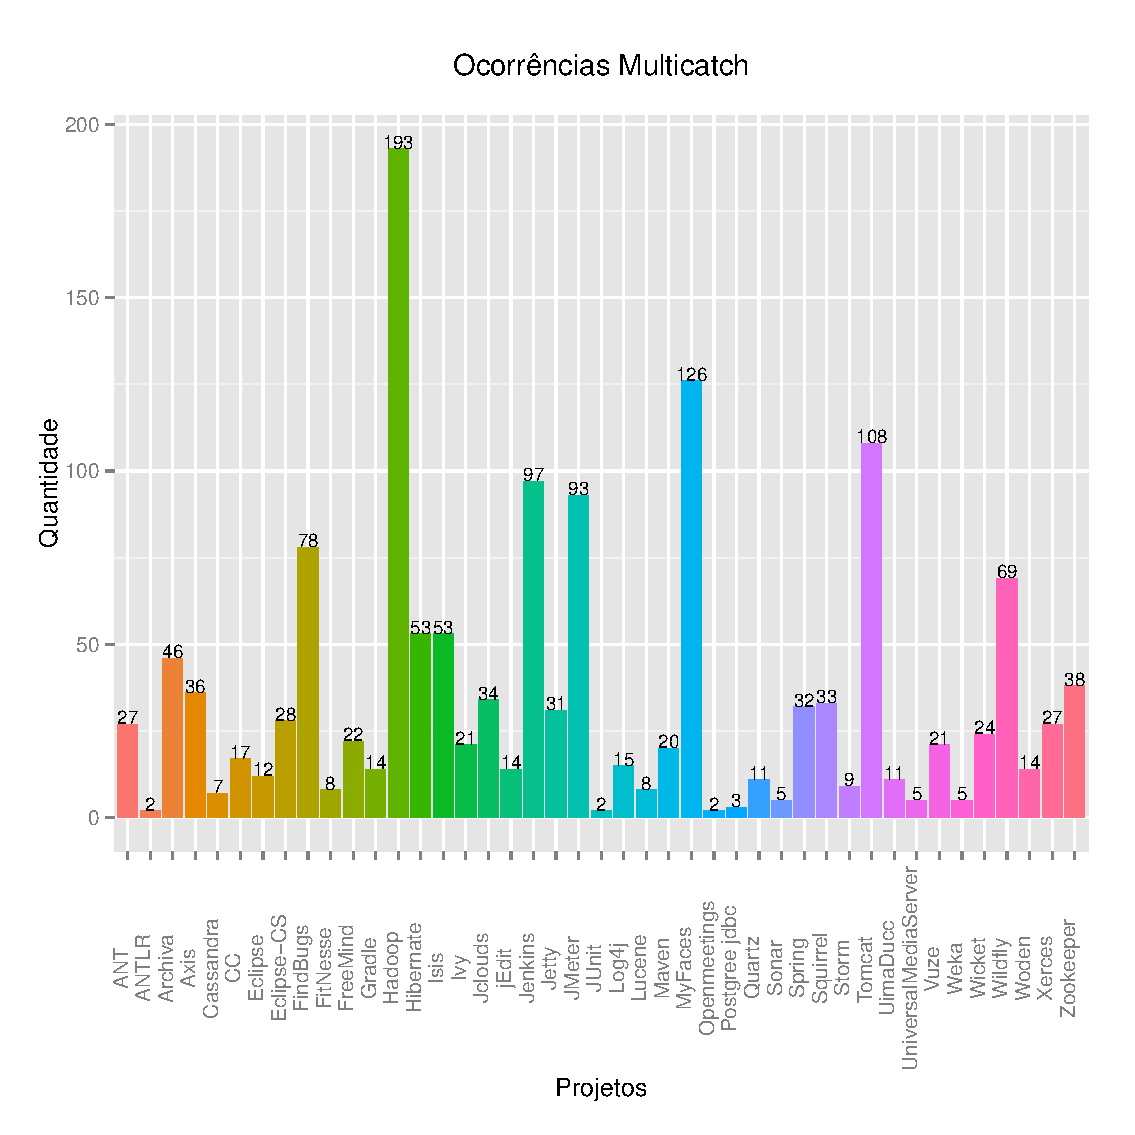
\includegraphics[scale=0.35]{../TCC/Imagens/ocorrenciasMulticatch}
				\label{fig:muticatch}
				\caption{Oportunidades de \texttt{multi-catch} nos projetos.}
			\end{figure}
		\end{block}
	
	\end{frame}	
%-------------------------------------------------------------------------------------------------	

% Try-Resource------------------------------------------------------------------------------------------------
	\begin{frame}[fragile, label=re]\frametitle{Resultados}
		\begin{block}{Try-Resource}
			\begin{itemize}
				\item Representam 1.15\% de todos os \texttt{try} dos sitemas.
			
				\item Encontrados 1616 ocorrências em 13 Projetos.
								
				\item \texttt{Server-Database} concentram 91\% das ocorrências.
			
			\end{itemize}
			
		\end{block}
		
	\end{frame}
	
	\begin{frame}[fragile, label=re]\frametitle{Resultados}
		\begin{block}{Try-Resource}
	
			\begin{figure}[Th]
				\center
				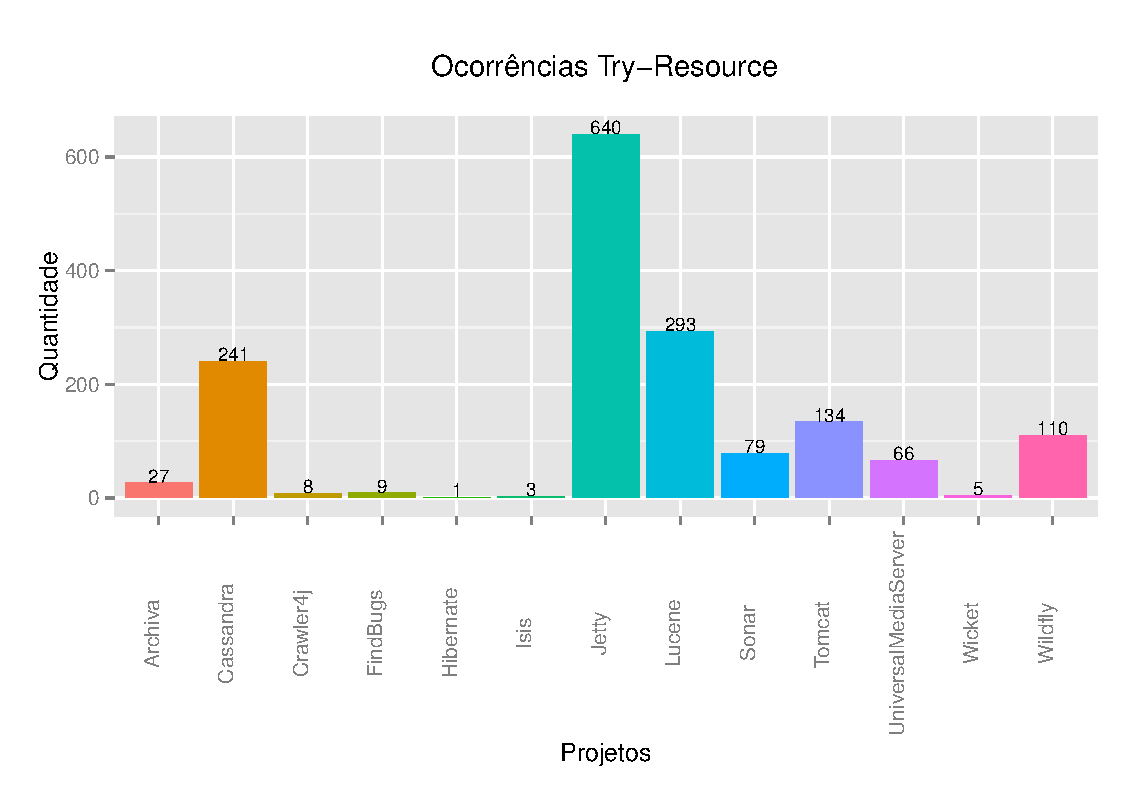
\includegraphics[scale=0.39]{../TCC/Imagens/ocorrenciasTryResource}
				\label{fig:tryresource}
				\caption{Adoção de \texttt{Try-Resource} nos projetos.}
			\end{figure}
		\end{block}
	
	\end{frame}	
%-------------------------------------------------------------------------------------------------	
	
% Switch-String------------------------------------------------------------------------------------------------	
	\begin{frame}[fragile, label=re]\frametitle{Resultados}
		\begin{block}{Switch-String}
			Menos de 1\% dos  6827 \texttt{Switch} usam \texttt{String}.

			\begin{table}[ht!] \footnotesize
				\centering
				\caption{Adoção \texttt{Switch String} por tipo do sistema.}
				\begin{tabular}{cc}
					\hline
					Sistema & Ocorrências \\ 
					\hline \hline
					\texttt{Cassandra} & 14 \\ 
					\texttt{FindBugs} & 3 \\ 
					\texttt{Jetty} & 16 \\
					\texttt{Lucene} & 2 \\
					\texttt{Sonar} & 1 \\
					\texttt{Spring} & 2 \\
					\texttt{Tomcat} & 8 \\
					\texttt{UniversalMediaServer} & 18 \\
					\texttt{Wicket} & 1 \\
					\texttt{Wildfly} & 1 \\	 \hline
					\texttt{Total} & 66 \\ \hline
				\end{tabular}
				\label{tab:adocaoSwitchString} %std means summary of type declarations
			\end{table}
		\end{block}
	\end{frame}
	
	
	
	\begin{frame}[fragile, label=re]\frametitle{Resultados}
		\begin{block}{Switch-String}
			\begin{itemize}
				\item Pesquisa por \texttt{if(String.equals(""))}.
				\item Foram encontrados 4940 em 45 dos 46 sistemas.
				\item \texttt{Switch-String} mais eficiênte que \texttt{if}.
			\end{itemize}
			
			\begin{table}[h]
				\centering
				\caption{Oportunidade de aplicar \texttt{switch} por tipo de sistema.}
				\begin{tabular}{cc}
					\hline
					Natureza & Ocorrências \\ 
					\hline \hline
					\texttt{Application} & 1773 \\ 
					\texttt{Library} & 1881 \\ 
					\texttt{Servers - Database} & 1286 \\ \hline
					\texttt{Total} & 4940 \\ \hline
				\end{tabular}
				\label{tab:oportunidadesSwitchPorNatureza} %std means summary of type declarations
			\end{table}
			
		\end{block}
	\end{frame}
	
	\begin{frame}[fragile, label=re]\frametitle{Resultados}
		\begin{block}{Switch-String}
			\begin{figure}[h]
				\center
				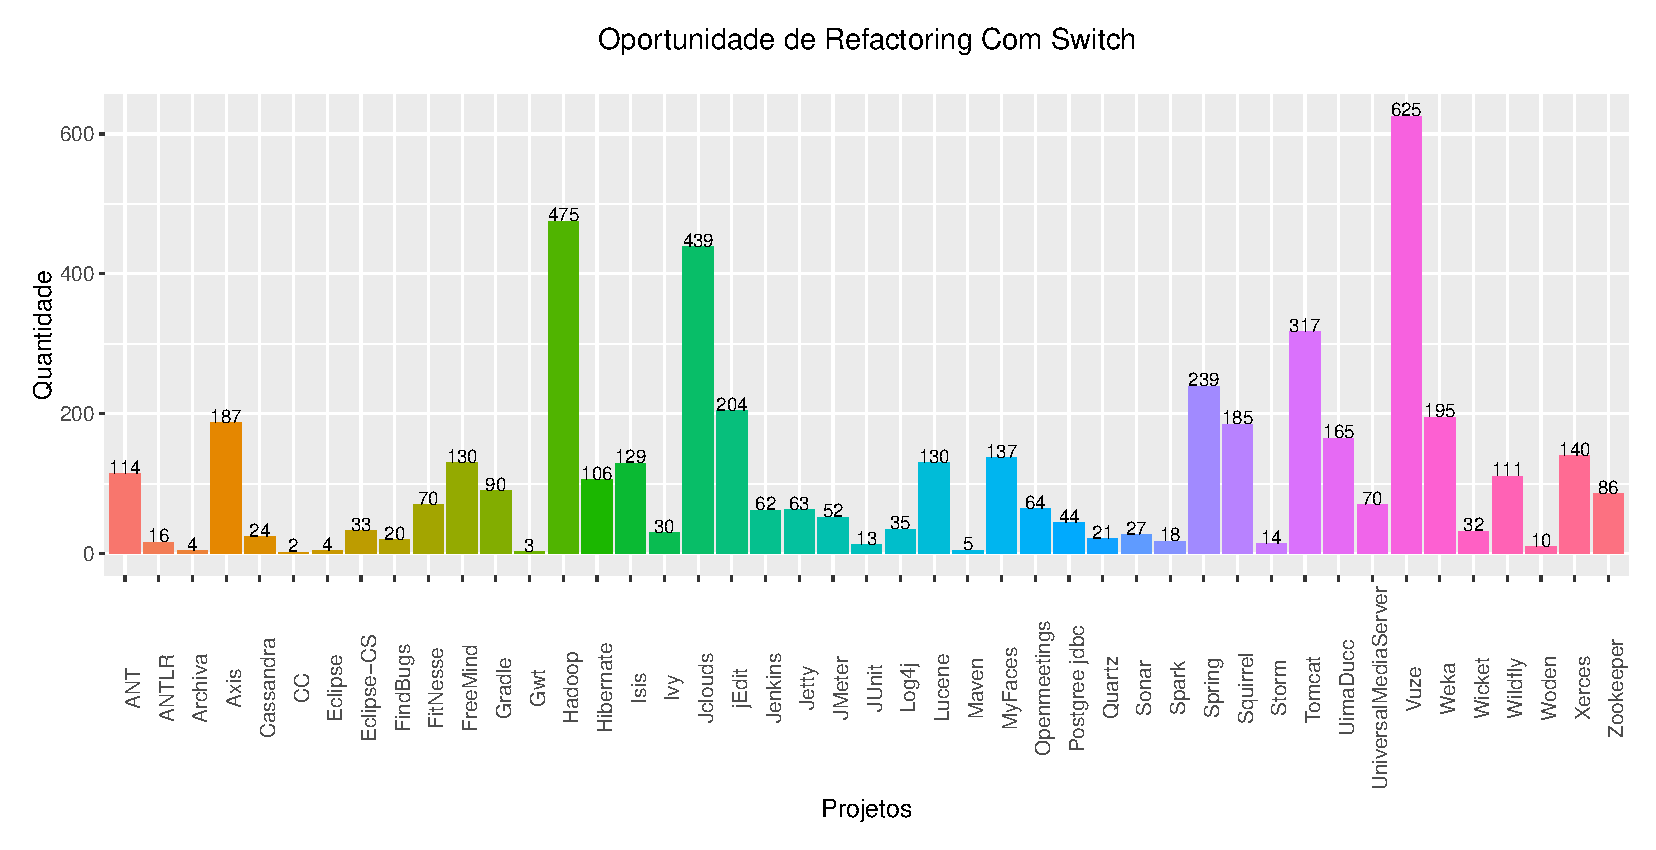
\includegraphics[scale=0.30]{../TCC/Imagens/oportunidadesSwitchString}
				\label{fig:oportunidadesSwitchString}
				\caption{Oportunidades de \textit{refactoring} em \texttt{if-then-else} por sistema.}
			\end{figure}		
		\end{block}
	\end{frame}
	
%e------------------------------------------------------------------------------------------------

% Conclusão ------------------------------------------------------------------------------------------------
	\begin{frame}[fragile, label=re]\frametitle{Conclusão}
		\begin{block}{Conclusão}
			\begin{itemize}
				\item Código obsoleto é mantido em versões atuais.
				\item Apesar da grande espectativa sobre Lambda, não existe um entusiasmo para adoção.
				\item A \texttt{realease} da linguagem não é importante no desenvolvimento.
				\item Temos um analisador flexível e estável para tentar automatizar \texttt{refactoring}.
			\end{itemize}
			
		\end{block}
	\end{frame}	


%%%%%%%%%%%%%%%%%%%%% Encerramento %%%%%%%%%%%%%%%%%%%%%
	\section{Encerramento}
	\begin{frame}[label=encerramento]
		\frametitle{Encerramento}
		\begin{block}{Perguntas}
			\centering
			\includegraphics[scale=0.6]{duvidas.jpg}\\
		\end{block}
	\end{frame}
%%%%%%%%%%%%%%%%%%%%% Encerramento %%%%%%%%%%%%%%%%%%%%%

\end{document}